\documentclass{article}

\usepackage[T1]{fontenc}
\usepackage[english]{babel}
\usepackage[utf8]{inputenc}
\usepackage{lmodern}
\usepackage{fullpage}

\usepackage{mathtools}
\usepackage{amsmath}

\usepackage{graphicx}
\usepackage{wrapfig}
\usepackage{caption}

\usepackage{biblatex}
\addbibresource{thesis.bib}

\title{An elementary analysis of the health board data}
\author{Henry Wilde}

\begin{document}

\maketitle




\section{Introduction}\label{section:intro}

The contents of this document forms a basis for much of the data analysis and
mining techniques to come in the writing of this thesis. The data itself is
provided by the cwm taf university health board and is comprised of patient
records from across several nhs trusts in south wales. \\

As of December 2017, the dataset contains 2,447,475 patient records described by
259 attributes. These attributes are a mix of categorical, numerical, binary and
datetime variables that include: personal identifiers like age and gender; cost
components; clinical variables like current diagnoses, severity of diagnoses,
treatment site, length of stay, and procedures undertaken. \\

This analysis is themed largely on costs as this is the primary focus of the
thesis. As such, many of the plots will be against cost components or attributes
known to have a strong correlation with cost of treatment like length of stay.
However, before any analysis is done, it is important to understand the data we
are dealing with. In this section, we will define the attributes which describe
the dataset, as well as how the data has been cleaned to make it relatively
uniform. 


\subsection{Attributes}\label{subsection:attributes}

Of the 259 attributes, 104 of them are indicators of the presence of numerous
conditions as well as Charlson index scores to measure the severity of a
comorbidity. As there are several thousand different primary diagnoses present, 
belonging to roughly one thousand HRGs, and no immediate way of grouping those
together in a sensible way, we will not be considering any comparative analysis
between conditions or procedures except for those documented in the existing
literature. \\

The remaining 155 attributes are made up of roughly 30 attributes for various
component costs of treating a patient (ward costs, imaging, critical care,
etc.), and the rest are either personal identifiers (age, gender, ID numbers) or
more general clinical attributes such as start and end wards, length of stay,
treatment site, consultant, registered GP practice, or admission method. These
are the attributes we will focus this elementary analysis on.


\subsection{Formatting the data}\label{subsection:formatting}

After receiving the dataset, a substantial amount of preprocessing was done to
make certain attributes -- and groups of attributes -- consistent, as well as
removing a number of extra attributes which were added after data collection
that provided no additional information. \\

A bit on what was actually done and why.


\section{Summative statistics}\label{section:summative}

As was discussed in Section \ref{subsection:attributes}, a large proportion of 
the attributes will not be considered in this analysis due to the volume of
values the attributes take. However, cost components and non-specific clinical
attributes are of interest. \\

When looking at this subset of attributes we can see that the data is heavily 
skewed toward short-stay, low-cost episodes and spells. The probability
density functions for length of stay and net cost are illustrated in Figures 
\ref{fig:LOS-kde} \& \ref{fig:NetCost-kde}, respectively, and show the extreme
nature of this skewedness.

\begin{figure}[h]
	\centering
	\begin{minipage}{.5\textwidth}
		\centering
		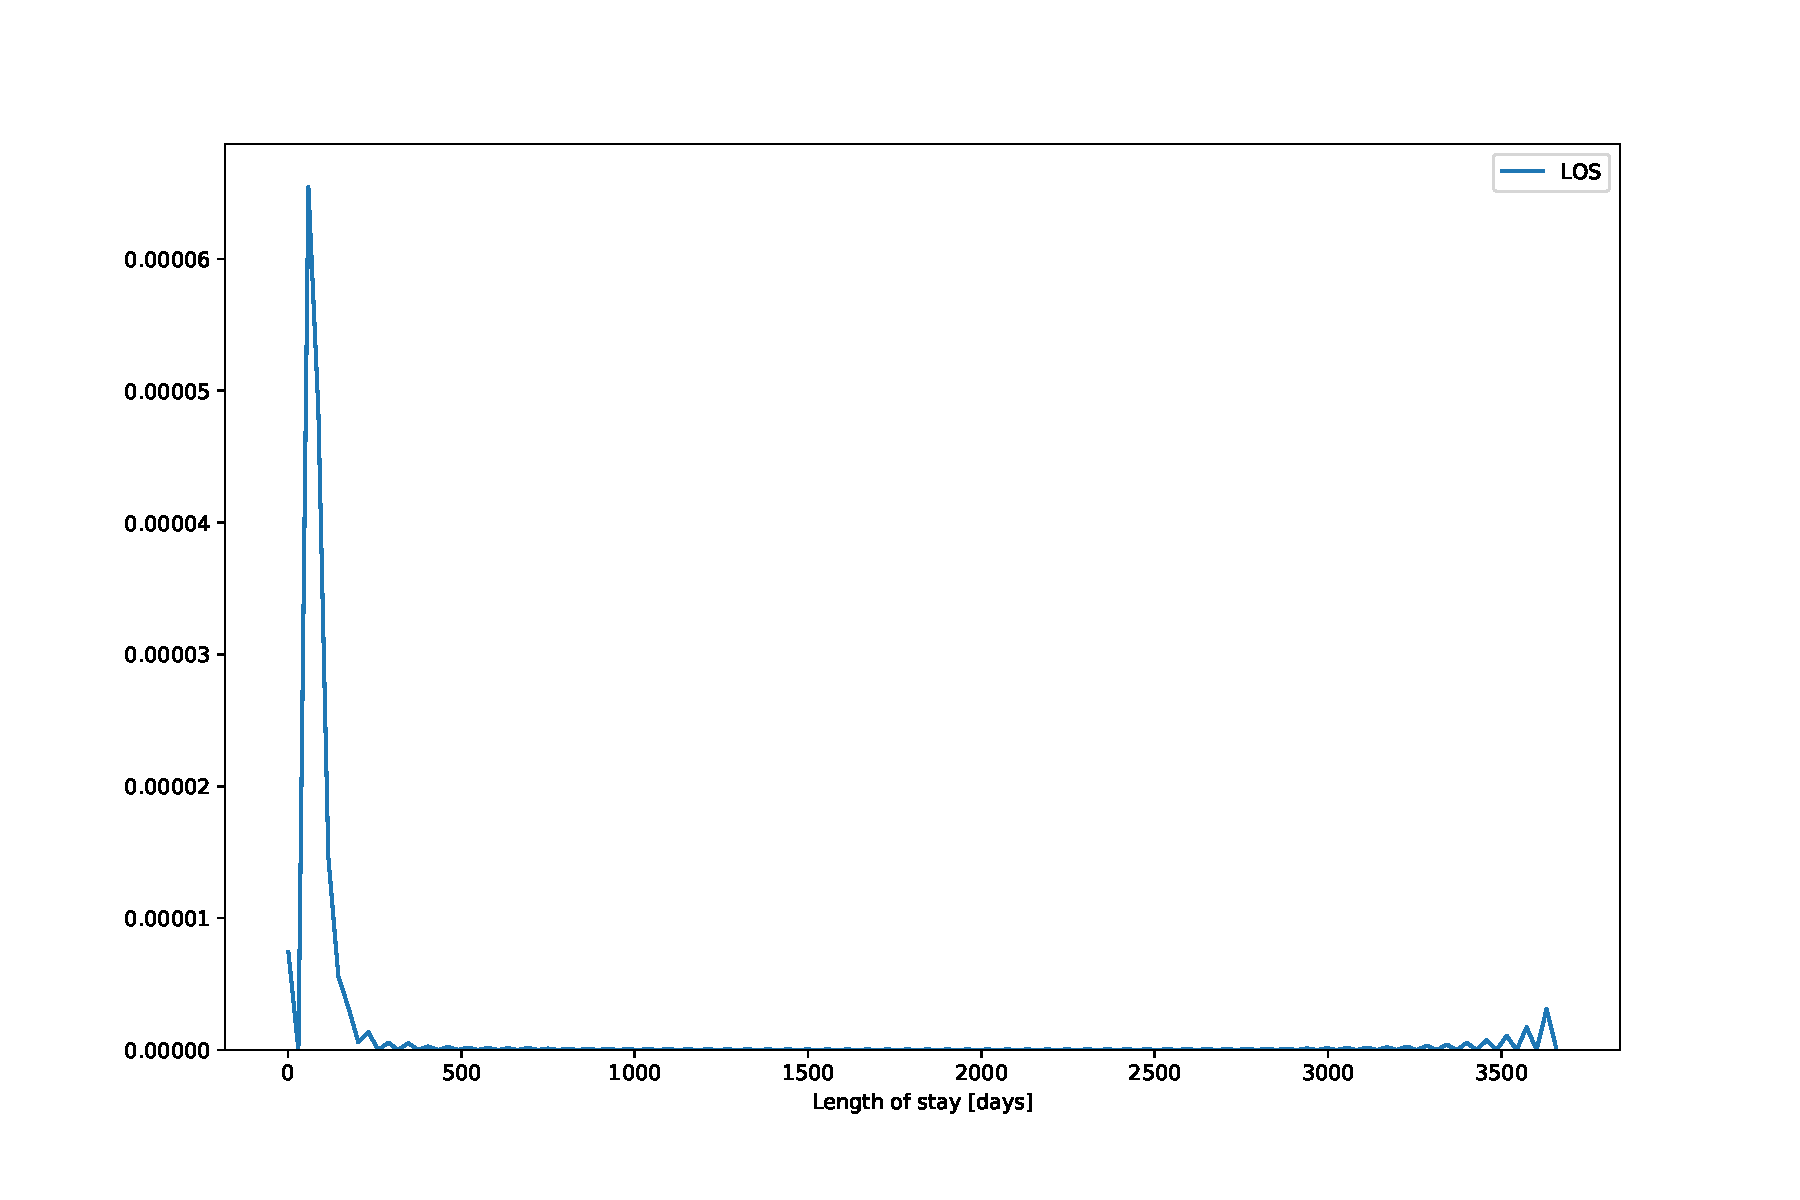
\includegraphics[width=\linewidth]{LOS-kde.pdf}
		\captionof{figure}{Estimated p.d.f. for length of stay.}
		\label{fig:LOS-kde}
	\end{minipage}%
	\begin{minipage}{.5\textwidth}
		\centering
		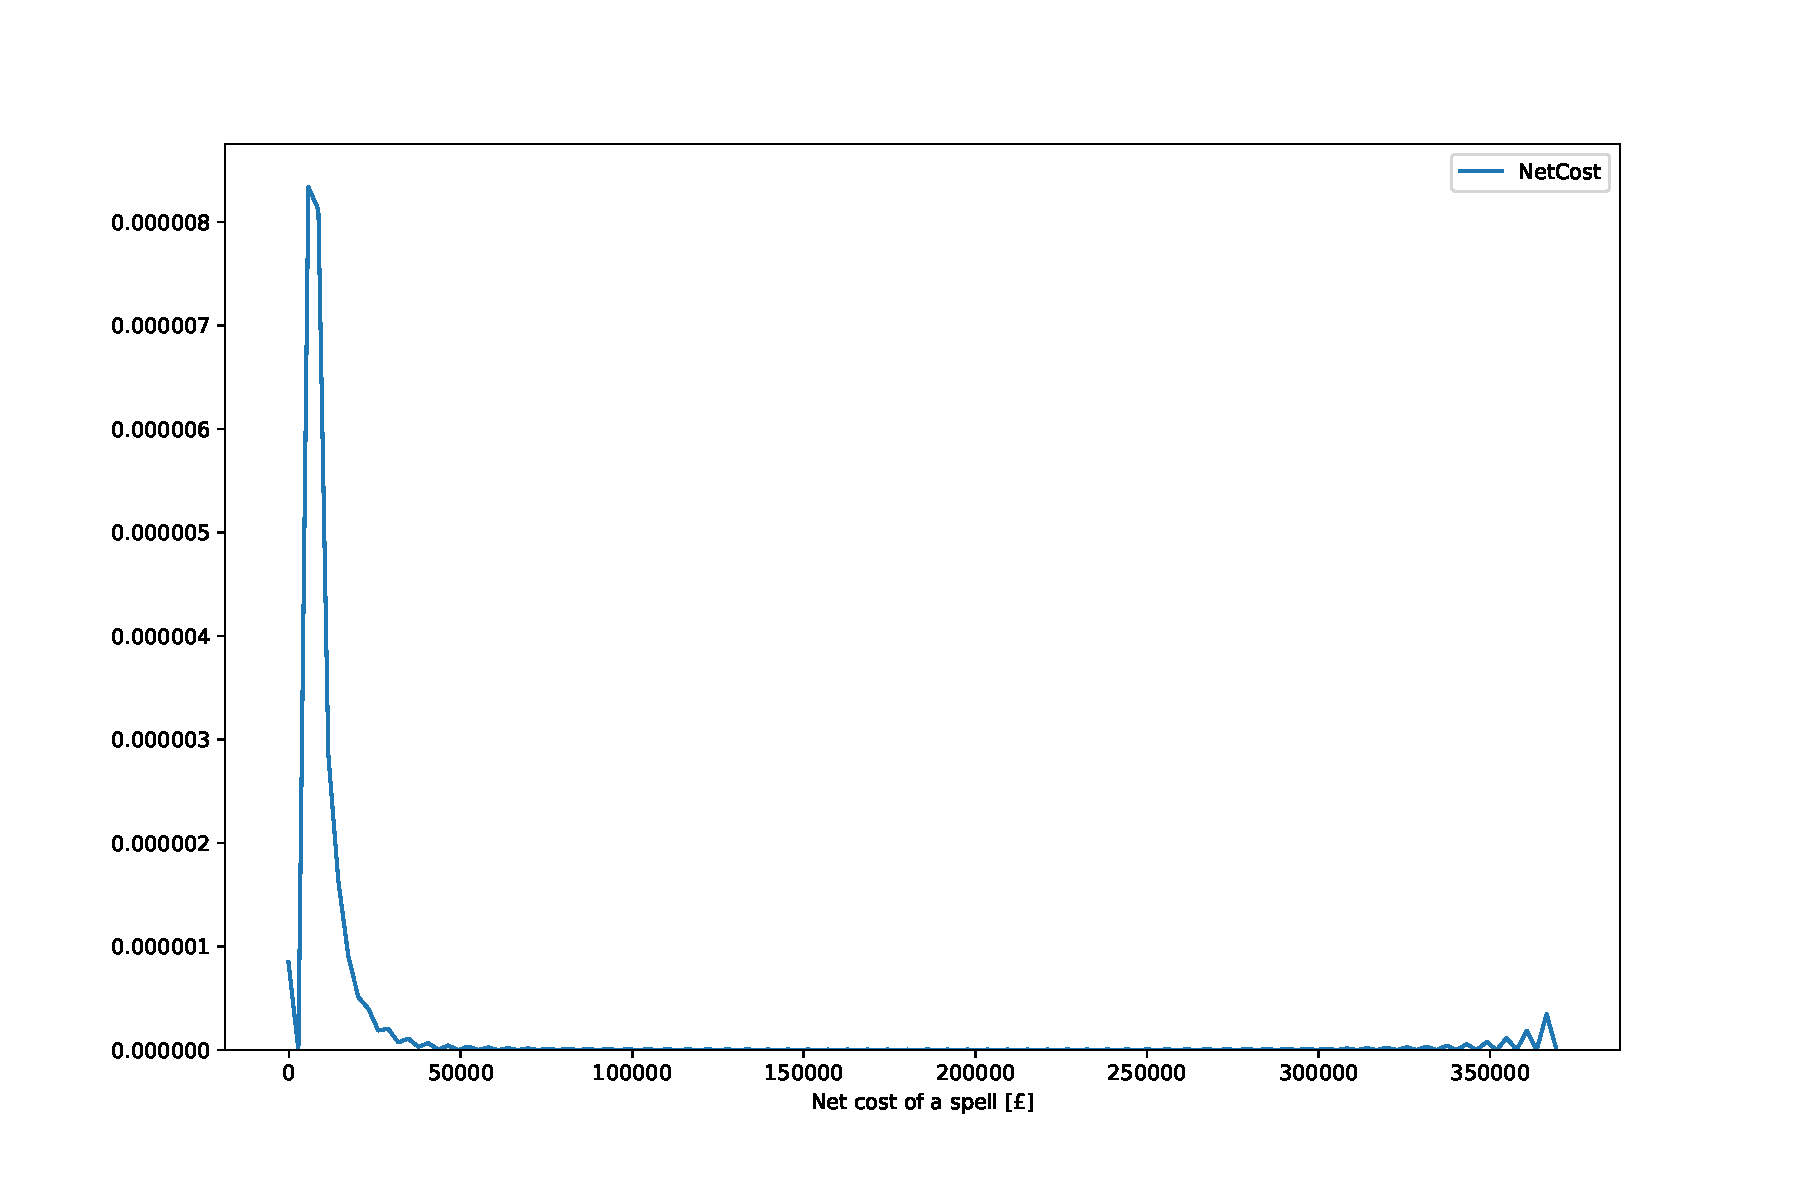
\includegraphics[width=\linewidth]{NetCost-kde.pdf}
		\captionof{figure}{Estimated p.d.f. for net cost.}
		\label{fig:NetCost-kde}
	\end{minipage}
\end{figure}

\begin{wrapfigure}{r}{.4\textwidth}
	\centering
	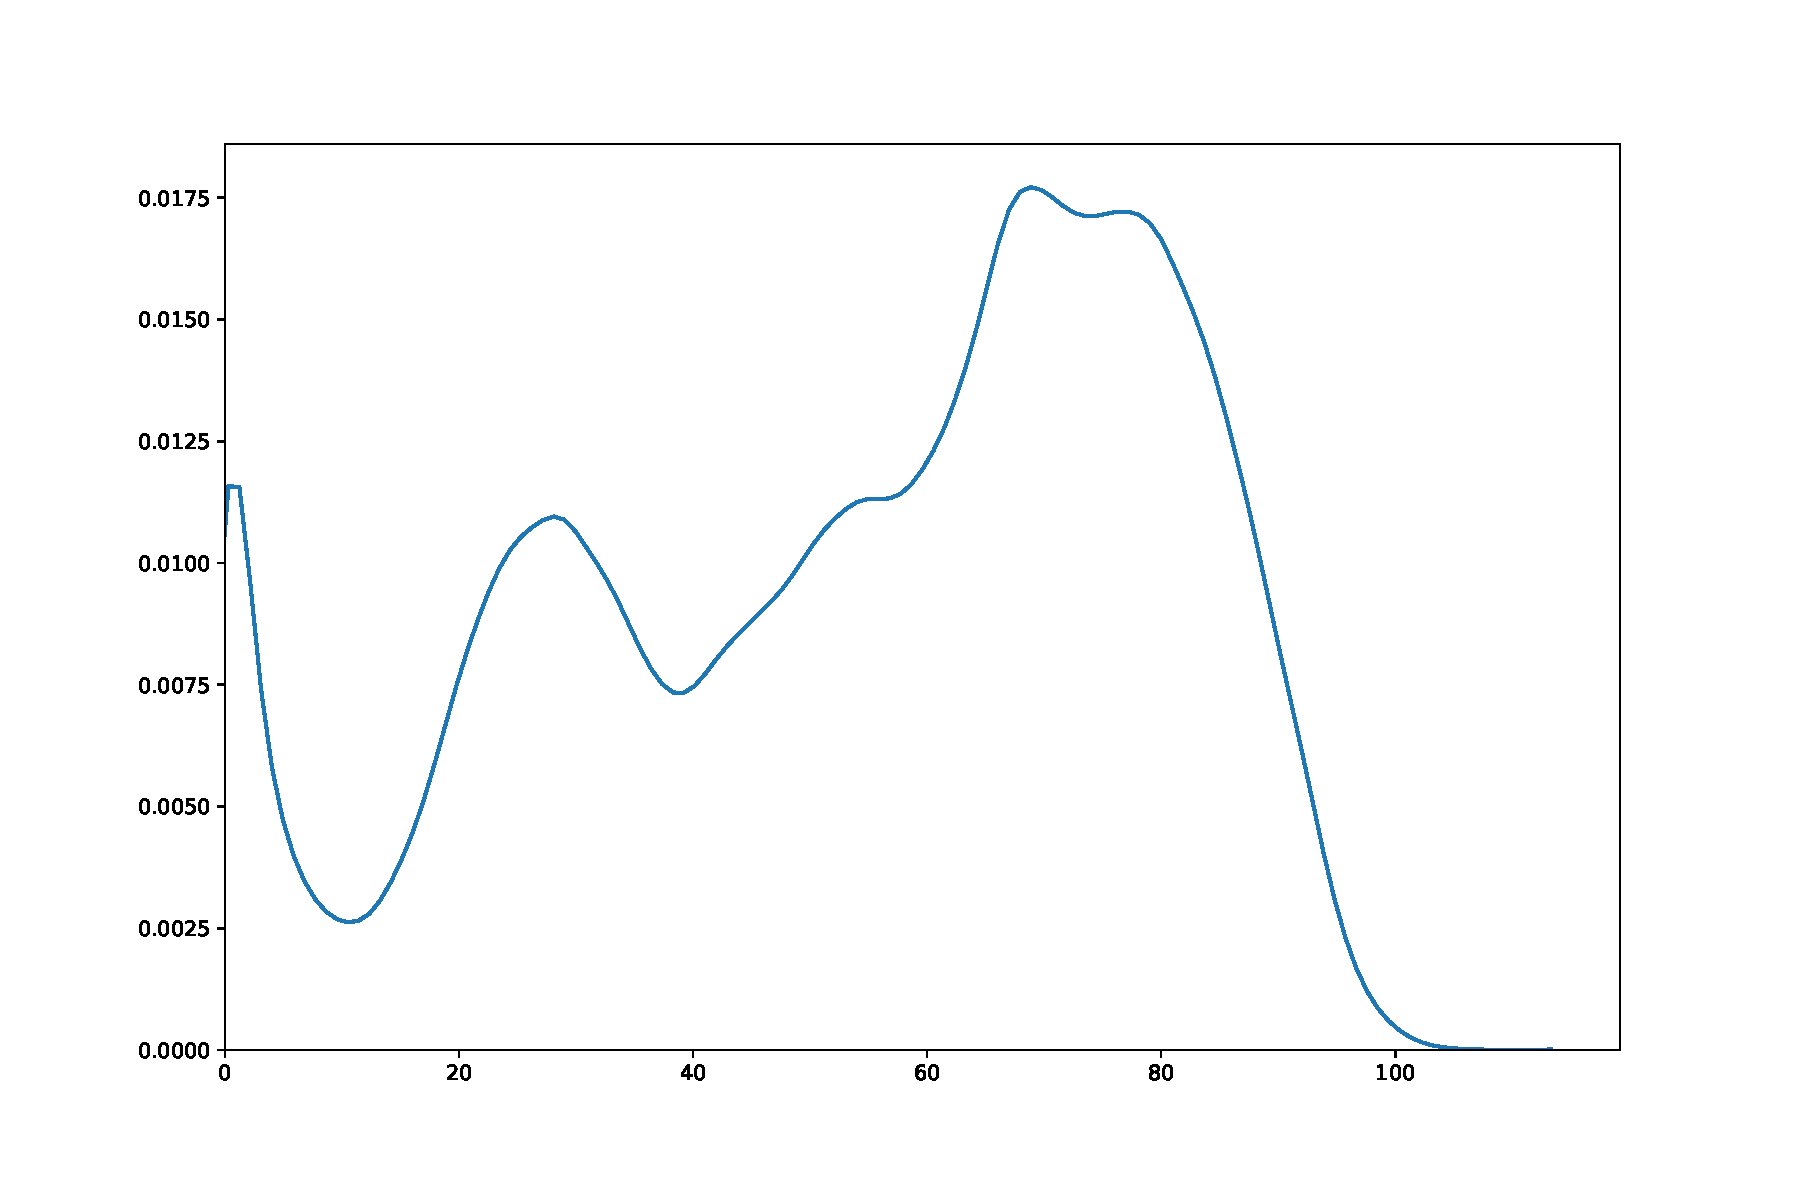
\includegraphics[width=\linewidth]{Age-kde.pdf}
	\caption{Estimated p.d.f. for age.}
	\label{fig:Age-kde}
\end{wrapfigure}

This skewedness could be tackled either by means of scaling the data or some
other transformation of certain attributes, but that is not to say that 
all the attributes are so harshly skewed; Figure \ref{fig:Age-kde} shows the
estimated p.d.f. for the age of a patient which has several very clear peaks and
troughs. \\

Note also that costs, for instance, are not only skewed but very widely spread.
In Figure \ref{fig:mean-cost-by-site} we see that average net costs are 
relatively stable across the two hospitals but even by one standard deviation, 
they are drastically different from the mean. These results can also be inferred
from Table \ref{table:stats}.

\begin{figure}[h]\label{fig:mean-cost-by-site}
	\centering
	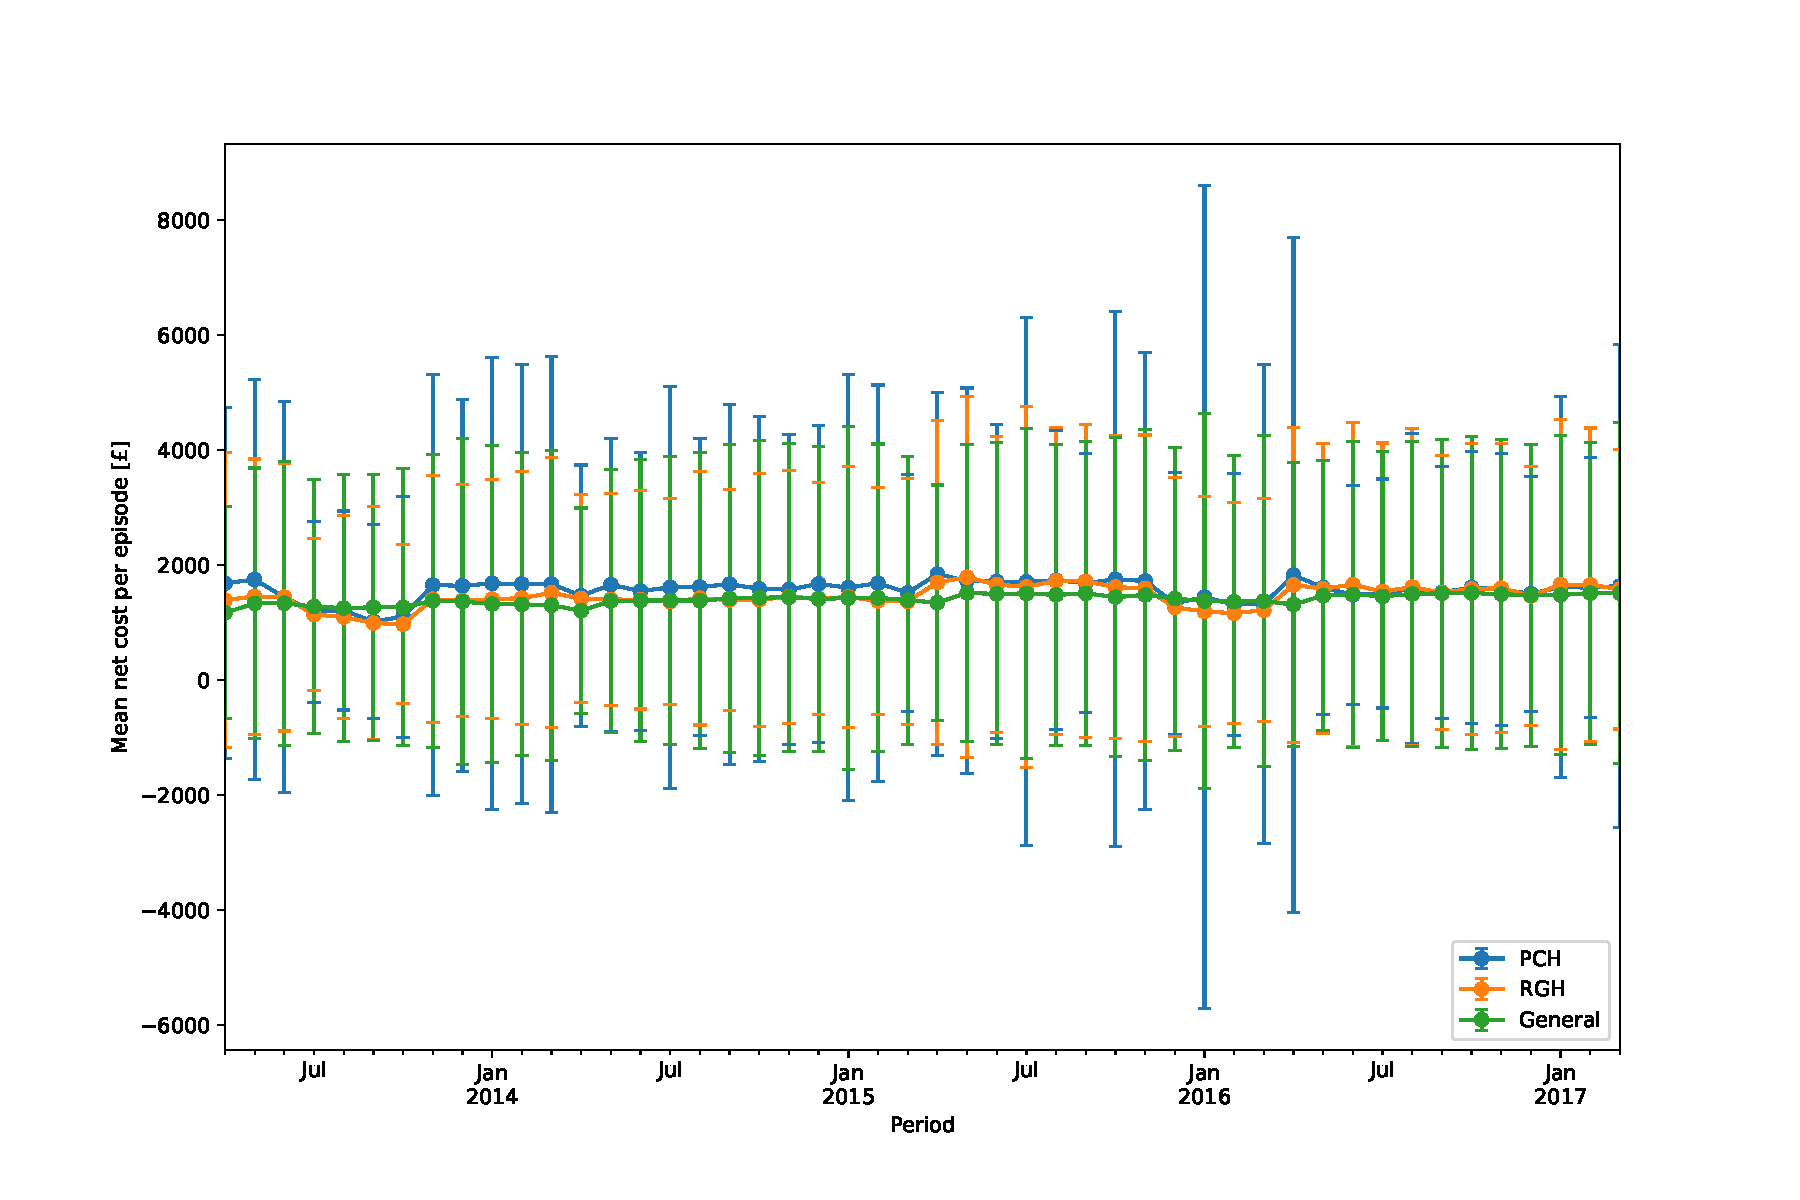
\includegraphics[width=.667\linewidth]{Mean-NetCost-by-site.pdf}
	\caption{Average net cost per episode between April 2013 and March 2017, 
	split across Prince Charles Hospital, Royal Gwent Hospital and all 
	records, including those without a specific treatment site.}
\end{figure}


\subsection{Summative statistics of selected attributes}
\label{subsection:summative}

Refer to Table \ref{table:stats} for some basic statistics describing the 
attributes selected above. Note that, again, we can see the skewedness of our 
data by examining the sudden increase in values across the interquartile range. 
\\

This is not wholely surprising given that, in an anecdotal way, we would expect 
the `average' patient in a given NHS system will be there for a short period of 
time with some smaller (and probably less expensive) condition. The larger and 
more extreme values likely come from the cost of scheduled, expert work or more 
elongated forms of care.

\begin{table}[h]
	\resizebox{\textwidth}{!}{%
	\begin{tabular}{l|c|c|c|c|c|c|c|c|c|c|c|c|c|c}
		{} & Age & Length of stay & No. procedures & No. diagnoses & 
		Net cost & Critical care & Medical & Ward & Blood & Pathology &
		Prosthetics & Imaging & Pharmacy & Overheads \\ 
		\hline
		Mean & 53.956 & 3.514 & 1.894 & 4.921 & 1742.39 & 92.30 & 346.95 
		& 497.04 & 2.06 & 36.23 & 40.66 & 32.69 & 30.48 & 354.79 \\
		\hline
		Std. dev. & 25.835 & 8.646 & 2.203 & 6.897 & 3181.09 & 1335.04 &
		740.13 & 1234.45 & 37.17 & 135.61 & 343.35 & 143.52 & 86.70 & 
		732.58 \\
		\hline
		Min. & 0 & 1 & 0 & 0 & 4.5 & 0 & 0 & 0 & 0 & 0 & 0 & 0 & 0 & 0 
		\\ 
		\hline
		25\% & 33 & 1 & 0 & 1 & 347.52 & 0 & 44.45 & 10.33 & 0 & 0 & 0 &
		0 & 2.26 & 84.86 \\ 
		\hline
		50\% & 59 & 1 & 1 & 3 & 747.39 & 0 & 130.67 & 142.22 & 0 & 4.67 
		& 0 & 0.08 & 7.26 & 139.61 \\ 
		\hline
		75\% & 75 & 2 & 3 & 6 & 1863.95 & 0 & 375.08 & 463.95 & 0.15 & 
		31.93 & 0 & 10.93 & 26.29 & 321.76 \\ 
		\hline
		Max. & 109 & 3659 & 58 & 455 & 369168.90 & 250000.60 & 116449.90
		& 203854.10 & 13768.71 & 70008.12 & 68029.58 & 46708.66 & 
		25087.73 & 106428.60 \\
	\end{tabular}
	}
	\caption{Summative statistics for some of our cost components
	as well as other numerical attributes. Costs (\textsterling), lengths of
	stay (days) and numbers of procedure/diagnoses are all per spell.}
	\label{table:stats}
\end{table}


\subsection{Correlation between attributes}\label{subsection:corr-cov}

Table \ref{table:corr} shows the Pearson correlation coefficient for all pairs 
of our selected attributes (not including age).

\begin{table}[h]\label{table:corr}
	\resizebox{\textwidth}{!}{%
	\begin{tabular}{l|c|c|c|c|c|c|c|c|c|c|c|c|c}
		{} & Length of stay & No. procedures & No. diagnoses &  Net cost
		& Critical care & Medical & Ward & Blood & Pathology &
		Prosthetics & Imaging & Pharmacy & Overheads \\
		\hline
		Length of stay & 1.000 & 0.188 & 0.461 & 0.808 & 0.215 & 0.483 &
		0.816 & 0.138 & 0.418 & 0.034 & 0.260 & 0.625 & 0.848 \\
		\hline
		No. procedures & 0.188 & 1.000 & 0.138 & 0.334 & 0.112 & 0.339 &
		0.178 & 0.081 & 0.207 & 0.108 & 0.272 & 0.172 & 0.236 \\
		\hline
		No. diagnoses & 0.461 & 0.138 & 1.000 & 0.407 & 0.099 & 0.206 & 
		0.427 & 0.102 & 0.292 & -0.002 & 0.216 & 0.377 & 0.442 \\
		\hline
		Net cost & 0.808 & 0.334 & 0.407 & 1.000 & 0.273 & 0.751 & 0.863
		& 0.177 & 0.480 & 0.217 & 0.308 & 0.673 & 0.910 \\
		\hline
		Critical care & 0.215 & 0.112 & 0.099 & 0.273 & 1.000 & 0.443 & 
		0.059 & 0.110 & 0.383 & 0.008 & 0.139 & 0.244 & 0.273 \\
		\hline
		Medical & 0.483 & 0.339 & 0.206 & 0.751 & 0.443 & 1.000 & 0.435 
		& 0.165 & 0.384 & 0.135 & 0.188 & 0.446 & 0.594 \\
		\hline
		Ward & 0.816 & 0.178 & 0.427 & 0.863 & 0.059 & 0.435 & 1.000 &  
		0.108 & 0.350 & 0.055 & 0.229 & 0.585 & 0.853 \\
		\hline
		Blood & 0.138 & 0.081 & 0.102 & 0.177 & 0.110 & 0.165 & 0.108 & 
		1.000 & 0.165 & 0.022 & 0.050 & 0.124 & 0.149 \\
		\hline
		Pathology & 0.418 & 0.207 & 0.292 & 0.480 & 0.383 & 0.384 & 
		0.350 & 0.165 & 1.000 & 0.014 & 0.223 & 0.382 & 0.431 \\
		\hline
		Prosthetics & 0.034 & 0.108 & -0.002 & 0.217 & 0.008 & 0.135 & 
		0.055 & 0.022 & 0.014 & 1.000 & 0.058 & 0.029 & 0.073 \\
		\hline
		Imaging & 0.260 & 0.272 & 0.216 & 0.308 & 0.139 & 0.188 & 0.229 
		& 0.050 & 0.223 & 0.058 & 1.000 & 0.216 & 0.254 \\
		Pharmacy & 0.625 & 0.172 & 0.377 & 0.673 & 0.244 & 0.446 & 0.585
		& 0.124 & 0.382 & 0.029 & 0.216 & 1.000 & 0.645 \\
		\hline
		Overheads & 0.848 & 0.236 & 0.442 & 0.910 & 0.273 & 0.594 & 
		0.853 & 0.149 & 0.431 & 0.073 & 0.254 & 0.645 & 1.000 \\
	\end{tabular}
	}
	\caption{Pearson correlation coefficients}
\end{table}

There are several attributes (such as Blood or Imaging) that have no significant
linear correlation with any of the other attributes but it is worth noting that
there are clear correlations between many of the attributes; some of these are
easier to realise than others. For instance, the longer the patient stays in a
hospital, the longer they will likely be on the ward. This is why we see a 
strong positive correlation between ward costs and length of stay. Similarly, 
the longer a patient is on a ward for, the more overheads (like meals) they 
incur.



\section{Known areas of interests}\label{section:known}

Given the amount of literature available around the following sections as well
as the works previously completed by the health board, we should attempt to
understand how the attributes associated with them settle in the data.

\subsection{Diabetes}\label{subsection:diabetes}

Can we see immediately what separates patients with diabetes (primary or
secondary) from those without? Do clusters exist in costs for those with and
without?

\begin{wrapfigure}{r}{.3\textwidth}\label{fig:diabetes-pie}
	\centering
	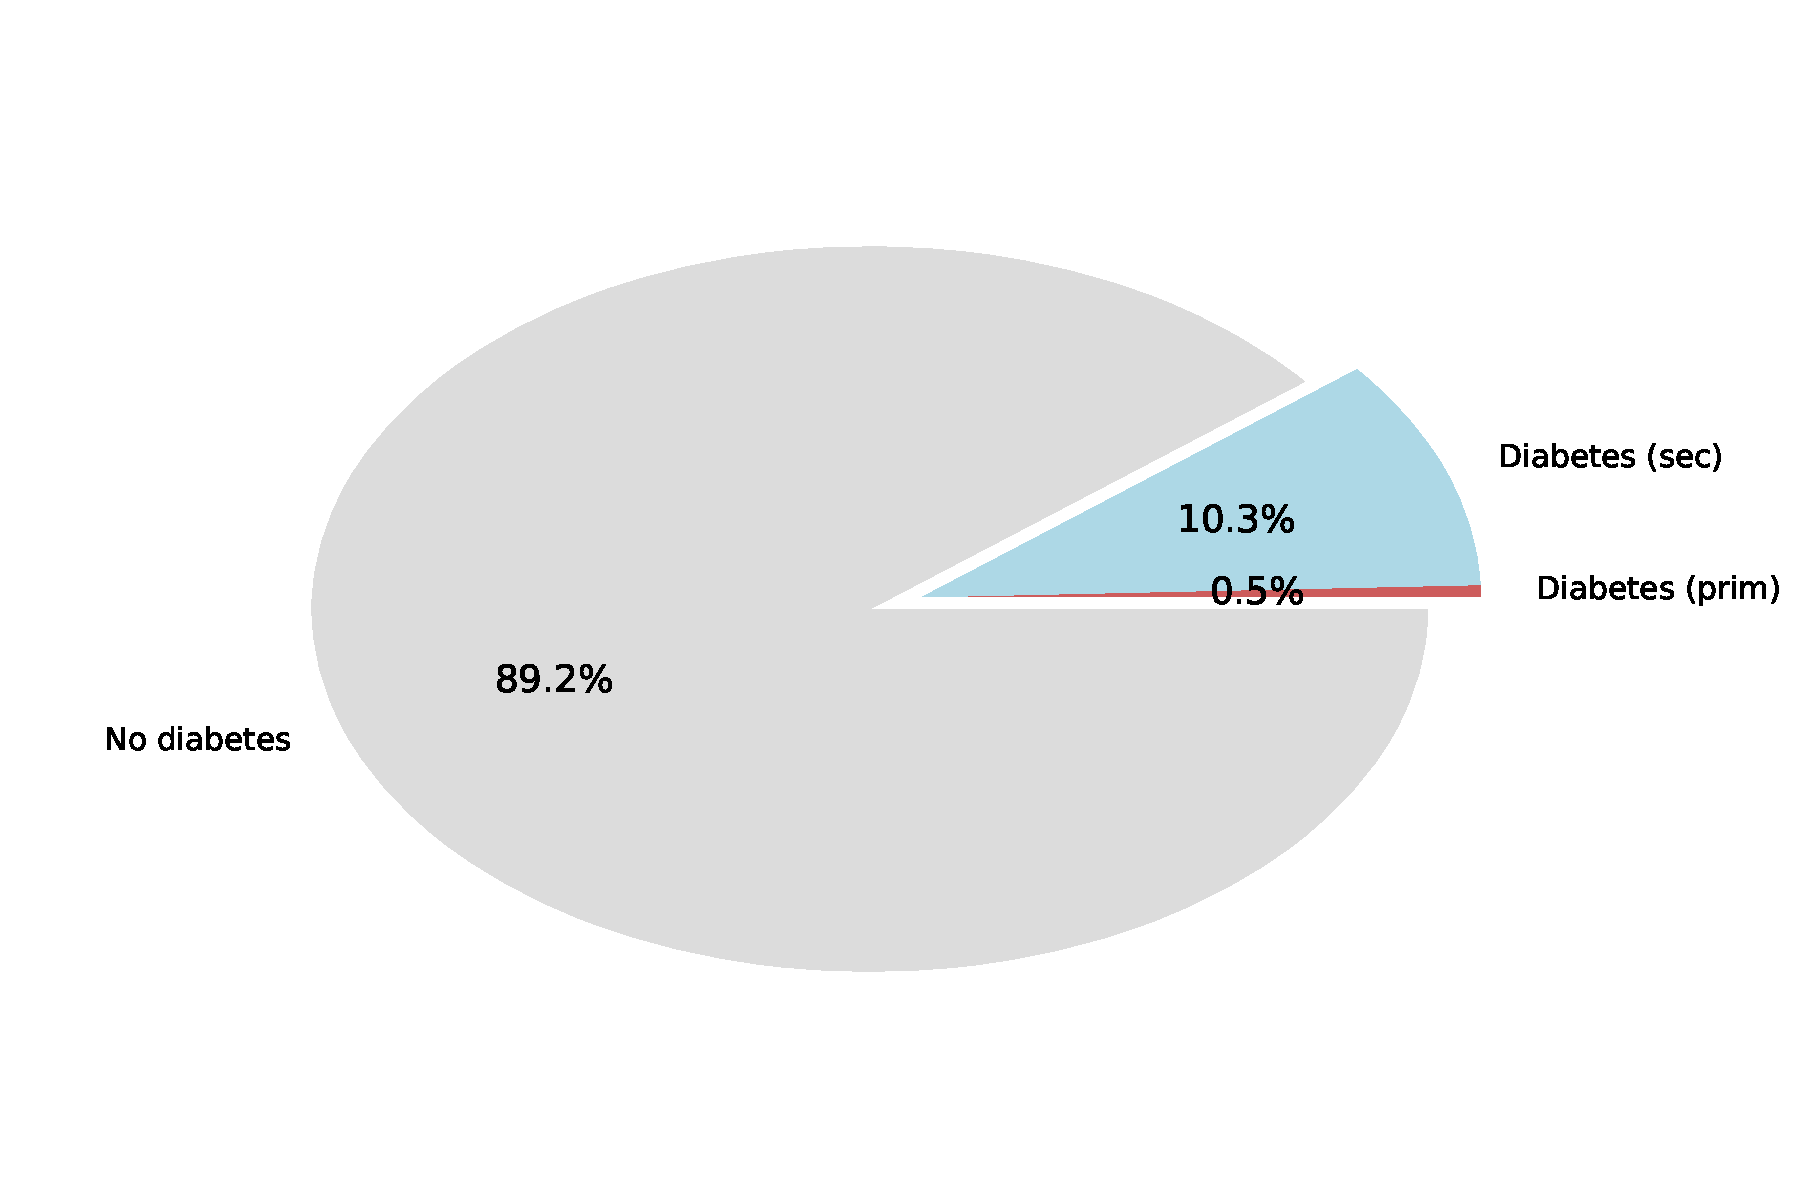
\includegraphics[width=\linewidth]{Diabetes-pie-chart.pdf}
	\caption{Percentage of patients being treated with diabetes (either as
	the primary or secondary condition) and those not.}
\end{wrapfigure}

\begin{table}[h]\label{table:diabetes-stats}
	\resizebox{\textwidth}{!}{
	\begin{tabular}{l|c|c|c|c|c|c|c|c|c|c|c|c|c|c}
		{} & Age & Length of stay & No. procedures & No. diagnoses & 
		Net cost & Critical care & Medical & Ward & Blood & Pathology & 
		Prosthetics & Imaging & Pharmacy & Overheads \\
		\hline
		Mean & 69.621 & 6.425 & 2.055 & 11.216 & 2656.44 & 152.78 & 
		443.67 & 846.55 & 4.24 & 64.24 & 54.46 & 57.97 & 58.46 & 580.28 
		\\
		\hline
		Std. dev. & 15.594 & 11.736 & 2.587 & 10.498 & 4164.13 & 1543.92 
		& 825.35 & 1679.10 & 48.04 & 176.09 & 434.86 & 174.07 & 124.68 & 
		985.15 \\
		\hline
		Min. & 0 & 1 & 0 & 1 & 10.91 & 0 & 0 & 0 & 0 & 0 & 0 & 0 & 0 & 0 
		\\
		\hline
		25\% & 62 & 1 & 0 & 5 & 491.79 & 0 & 67.71 & 59.64 & 0 & 0.68 & 
		0 & 0 & 3.81 & 107.56 \\
		\hline	
		50\% & 72 & 2 & 2 & 8 & 1231.22 & 0 & 193.41 & 273.94 & 0 & 
		20.13 & 0 & 0.98 & 16.24 & 230.32 \\
		\hline
		75\% & 81 & 7 & 3 & 13 & 3113.81 & 0 & 478.93 & 989.11 & 0.51 & 
		71.03 & 0 & 38.26 & 71.78 & 665.51 \\
		\hline
		Max. & 107 & 678 & 43 & 423 & 273450.30 & 193076.19 & 58673.47 & 
		173963.47 & 5757.19 & 28621.00 & 28955.99 & 8097.57 & 14812.14 &
		57647.29 \\
	\end{tabular}
	}
	\caption{Summative statistics for our selected attributes specifically
	for those diagnosed with diabetes}
\end{table}

\begin{wrapfigure}{l}{.5\textwidth}\label{fig:diabetes-age-kde}
	\centering
	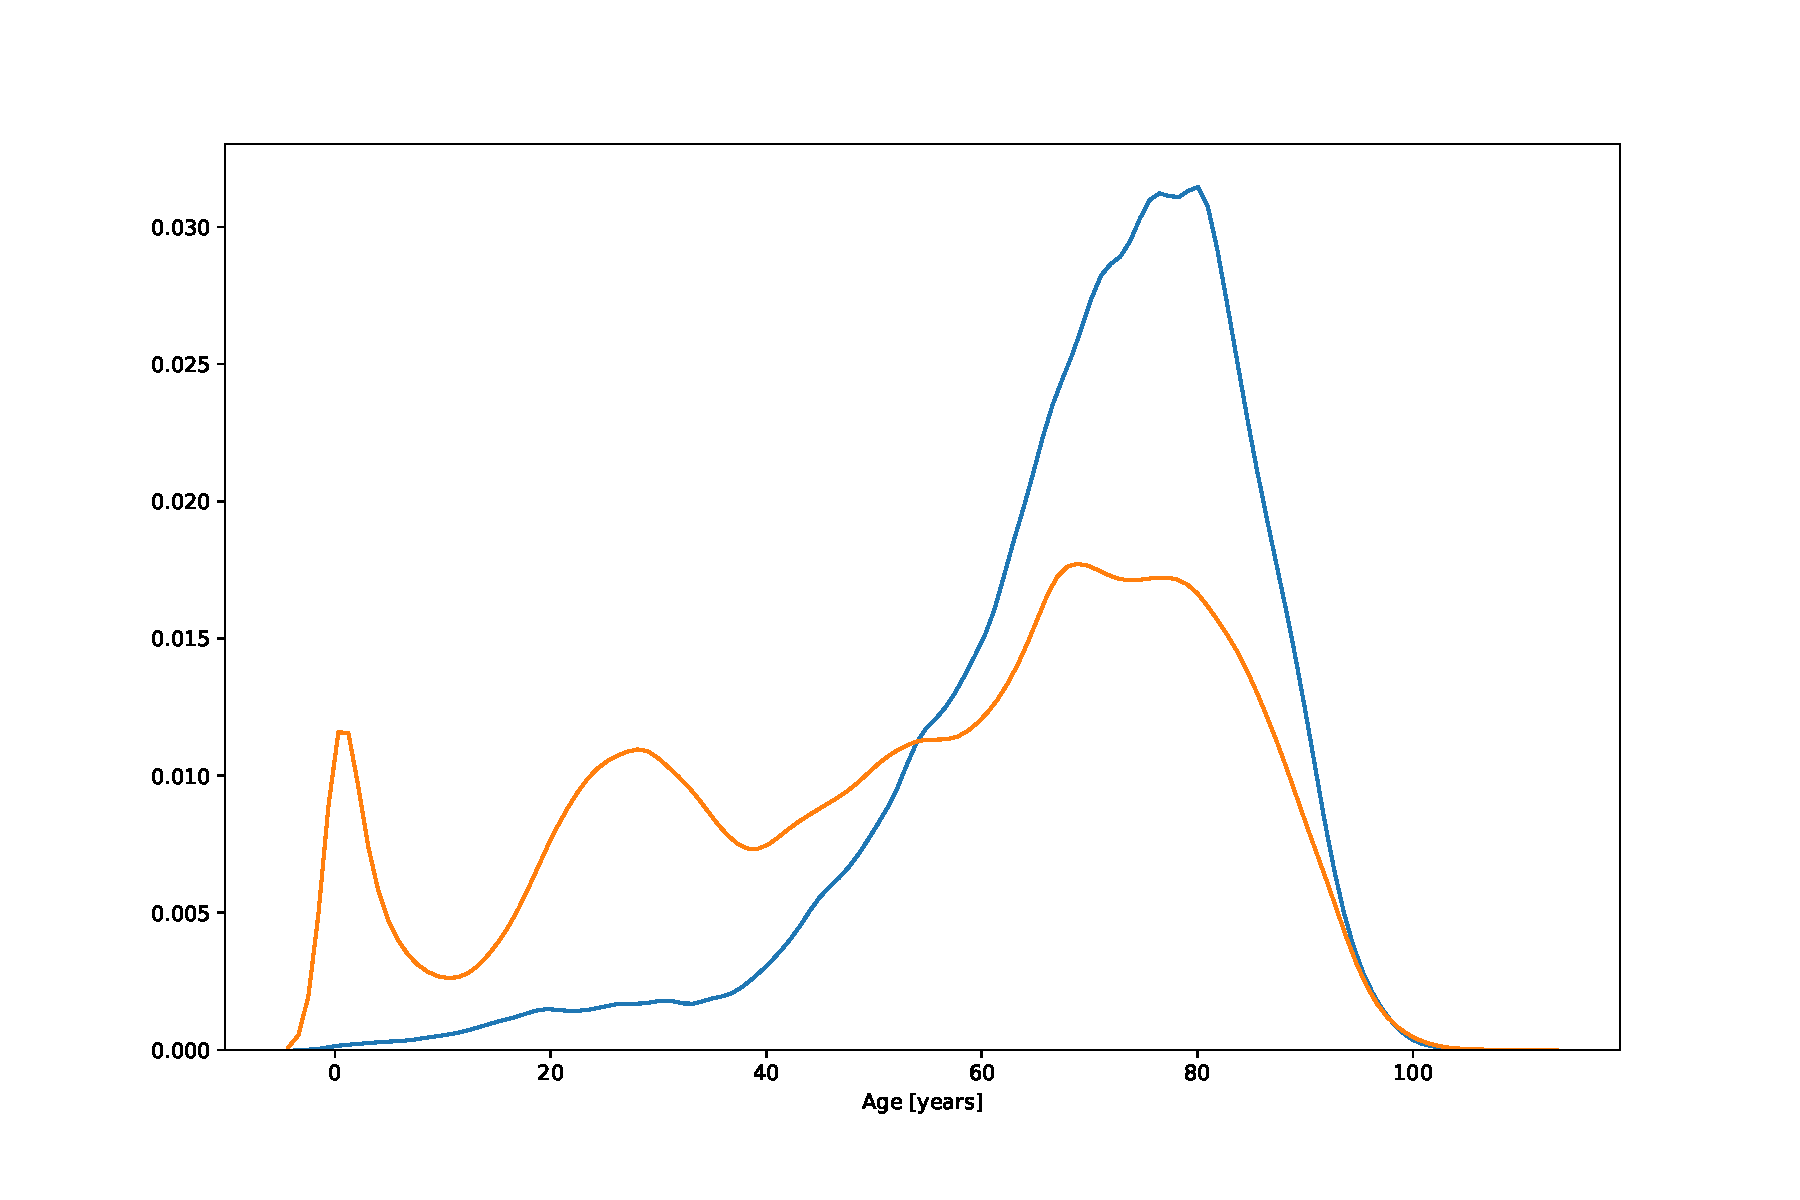
\includegraphics[width=\linewidth]{Diabetes-Age-kde.pdf}
	\caption{Estimated p.d.f. for the age of diabetic patients}
\end{wrapfigure}

\subsection{Ward}\label{subsection:ward}

Are the results from the paper reproducible with our data?


%\printbibliography
\end{document}
